%!TEX root = ../main.tex
\chapter{Introduction} \label{cap: introduction}
The gap between hard disk drives' (HDDs) performance and processors' computing power, better known as the I/O performance gap problem, represents a serious scalability limitation for scientific applications running on High End Computing (HEC) clusters. To address this problem, HEC clusters system software is built with multiple layers stacked on top of each other. These layers were added incrementally over the years to provide new features/optimizations, and to solve existing problems. Unfortunately, since the corresponding software components were not designed and built in an integrated manner, they often duplicate existing functionalities and introduce additional parameters that make the optimal configuration of the system a very difficult task. Figure~\ref{figure: hpc-io-stack} shows a typical layering for the High Performance Computing (HPC) I/O software stack.

\begin{figure}[!htb]
  \centering
  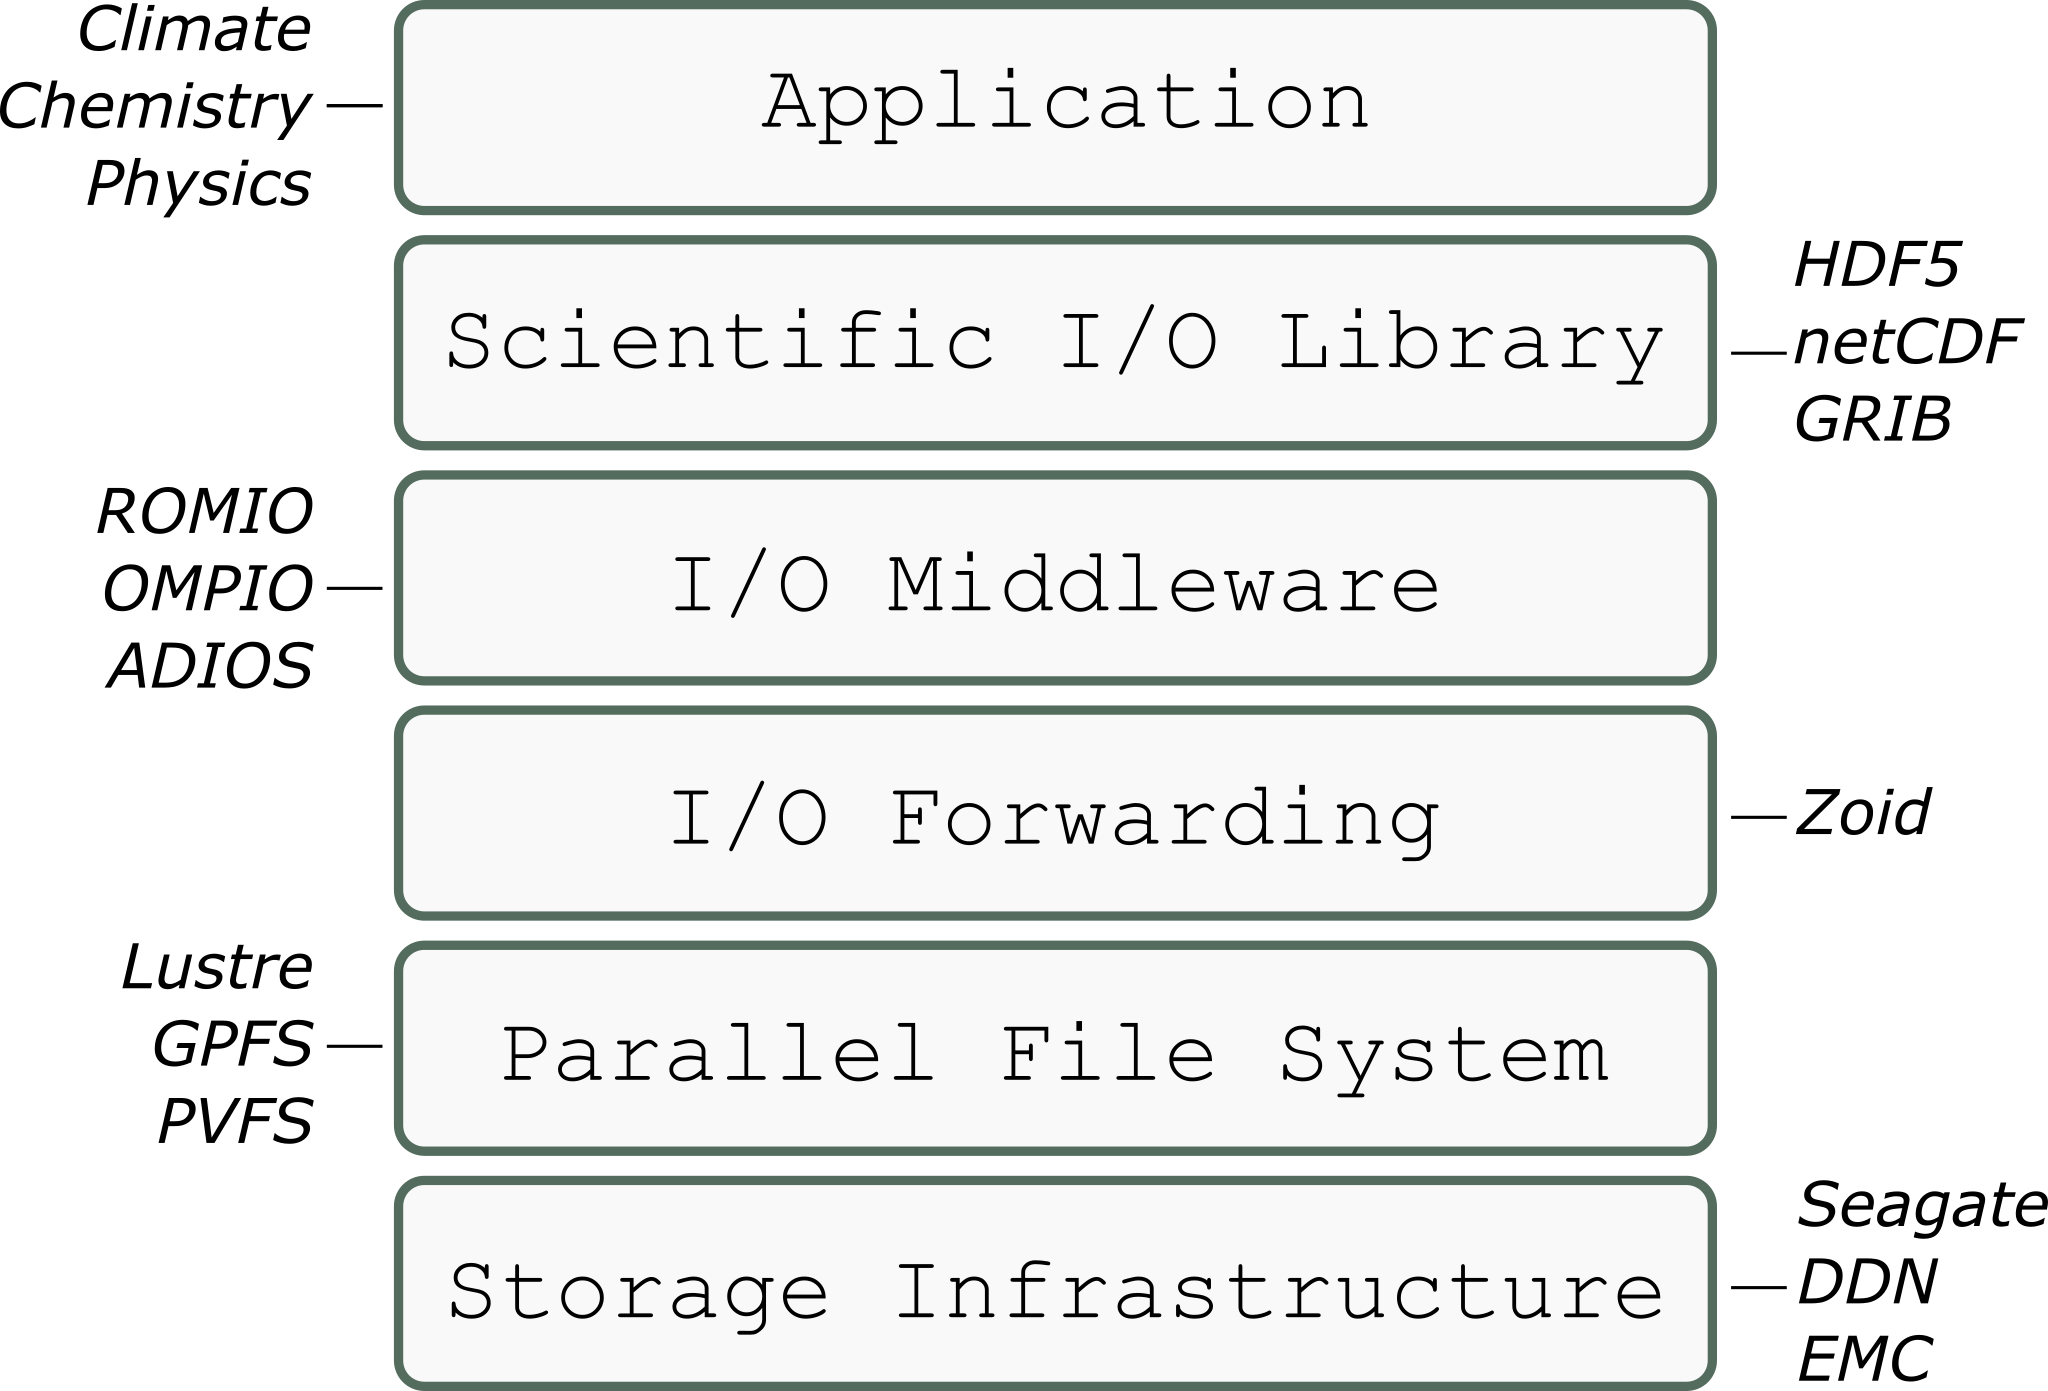
\includegraphics[width=0.6\textwidth]{chapters/figures/hpc-io-stack}
  \caption{HPC I/O Stack}
  \label{figure: hpc-io-stack}
\end{figure}

At the bottom of the stack in Figure~\ref{figure: hpc-io-stack} is the \textit{Storage Infrastructure} represented by vendor specific hardware/software solutions that aggregate and export data blocks from remote HDDs to the clients using a low latency Storage Area Network (SAN). The \textit{Parallel File System} software, on top of the Storage Infrastructure, consolidates these blocks into a more usable and familiar file interface. Parallel File Systems (PFSs) such as Lustre~\cite{Braam02}, PVFS~\cite{CarnsLRT} and GPFS~\cite{SchmuckH02}, just to mention a few, exploit the storage devices available on the network by striping files across them and providing clients with parallel paths to reach data, thus increasing the aggregated I/O bandwidth. Frequently storage vendors also provide the parallel file system software optimized for their hardware configuration (e.g. GPFS for IBM and custom Lustre for Seagate). The \textit{I/O Forwarding} layer is optionally used in some supercomputer designs, such as the IBM Blue Gene systems, to delegate file system access to a limited number of intermediate I/O clients, with the benefit of reducing the Operating System (OS) noise in the compute nodes~\cite{AliCIKLLRWS09}. The \textit{I/O Middleware} provides parallel I/O towards the underlying file system, typically using the MPI-IO interface to achieve high performance data access as well as consistency. ROMIO\footnote{Implementation of MPI-IO specifications from Argonne National Laboratory included in the MPICH package (\url{http://www.mpich.org})} is an example of popular I/O middleware used in HPC. It implements the MPI-IO extensions to the POSIX I/O interface, and through the Abstract Device I/O  (ADIO) drivers~\cite{ThakurGL96} enables transparent file access optimizations based on two-phase I/O and data sieving, adapting I/O patterns to the characteristics of the underlying file system~\cite{ThakurGL99}. However, MPI-IO does not provide applications with the infrastructure they need to organize and manage their data in a more abstract and efficient manner. Thus, \textit{Scientific I/O Libraries} have been introduced at the top of the stack to bridge the gap between how data is represented and organised at the application level (data model) and how it is mapped onto the underlying file system (storage model). Popular I/O libraries include the Hierarchical Data Format library (HDF5)~\cite{hdf5} and the network Common Data Format (netCDF)~\cite{netcdf}.

%\section{I/O Middleware Layer} \label{sec: io-middleware}
In this thesis we focus on the I/O middleware layer of the I/O software stack presented in Figure~\ref{figure: hpc-io-stack}. The I/O middleware represents a key component for achieving high performance in HPC since it connects the parallel file system to the high-level I/O libraries (most commonly HDF5 or netCDF). For this reason the I/O middleware is the best place to implement automatic and semi-automatic optimisations. Contextually, guided I/O interfaces can be used as effective mechanism to deliver the requested optimisation messages.

\section{Guided I/O Interfaces} \label{sec: guided-io}
Generally guided I/O interfaces come in the form of extensions to the standard API of the main software component. Users, as well as other software packages, can exploit these extensions to control the internal behaviour of the component, altering the way the standard API works. Guided I/O APIs are present at different levels in the I/O software stack but are most commonly found in the I/O middleware and the file system components.

\subsection{Guided I/O in MPI-IO} \label{subsec: mpi-io-hints}
The ROMIO middleware provides guided I/O support through the MPI-IO hints API, specifically designed to control internal ROMIO parameters and trigger different I/O optimisations. MPI-IO hints are packed into a special info object and passed down to the middleware through the MPI file open API. The MPI-IO hints mechanism allows the middleware to convert I/O patterns generated by applications into I/O patterns that are compatible with the characteristics of the underlying file system, thus improving I/O performance. In this way the same MPI file read and write operations can behave differently depending on the hints passed to the middleware when the file was opened. Specifically, if the collective I/O hint is enabled ROMIO will convert every non-contiguous independent write to the file into a smaller number of sequential coordinated writes.

Besides I/O pattern selection, MPI-IO hints can be also used to control the size of the buffers used by ROMIO when performing I/O, to select the stripe size used by the file system to store data across the available I/O servers and even to select the number of I/O servers used to store the file.

\subsection{Guided I/O in Linux File Systems} \label{subsec: posix-advice}
At the file system level the Linux kernel provides users with the capability to communicate access pattern information to the local file system through the \texttt{posix\_fadvise()}~\cite{AdviseAPI} system call. The file system can use this information to improve page cache efficiency, for example, by prefetching (or releasing) data that will (or will not) be required soon in the future or by disabling read-ahead in the case of random read patterns. %Nevertheless, \texttt{posix\_fadvise()} is barely used in practice and has intrinsic limitations that discourage its employment in real applications.

The two most used PFSs in HEC clusters nowadays, GPFS and Lustre, are both POSIX compliant. However, neither of them supports the POSIX advice mechanism previously described. GPFS compensates for the lack of POSIX advice support through a hints API that users can access by linking their programs against a service library. Hints are passed to GPFS through the \texttt{gpfs\_fcntl()}~\cite{GPFSHINTS} function and can be used to guide prefetching (or releasing) of file blocks in the page pool\footnote{GPFS pinned memory used for file system caching.}. Lustre, on the other hand, does not provide any client side mechanism similar to GPFS hints or POSIX advice.

\section{Opportunities with Non-Volatile Memories} \label{sec: nvm}
The availability of Solid State Drives (SSDs) and, more generally, Non-Volatile Memory (NVM) devices in the storage hierarchy provides new opportunities for optimisations based on data placement and migration across the different memory tiers of the system. Although HPC compute nodes have access to locally attached SSDs, these are rarely integrated in the I/O software stack. A possible way of integrating the new memory devices in the stack is given by guided I/O interfaces in the I/O middleware component. By using the guided I/O API in the middleware users can control data placement and migration to improve the efficiency of specific I/O patterns.

One practical use case for NVM devices is file caching. File caching can be useful in many different scenarios. Generally, caching can be used to reduce the I/O latency as well as the number of network requests generated by file system clients. More specifically, since the number of NVM devices can scale linearly with the number of compute nodes in the cluster, it can also improve the aggregated I/O bandwidth. Additionally, caching can be useful to improve collective I/O performance. Collective I/O is a parallel I/O technique in which write performance is highly dependent upon the storage system response time and limited by the slowest writer. The storage system response time in conjunction with the need for global synchronisation, required during every round of data exchange and write, severely impacts collective I/O performance. Future Exascale systems will have an increasing number of processor cores, while the number of storage servers will remain relatively small. Therefore, the storage system concurrency level will further increase, worsening the global synchronisation problem.

NVM file caching can alleviate the global synchronisation problem in collective I/O by minimising the I/O time variation across compute nodes and can increase the I/O bandwidth by aggregating together multiple NVM devices on different compute nodes.

\section{Contribution} \label{sec: contribution}
In the described context our work provides two main contributions. First, we bring the POSIX Advice and GPFS hints APIs together in a unified middleware component called Mercury~\cite{CongiuGPMSB}. Mercury exports a single API and can transparently select the appropriate underlying hints interface depending on the file system backend used to store the data. Additionally, we modify the Virtual File System (VFS) layer in the Linux kernel to enable the \texttt{posix\_fadvise()} system call for Lustre and more generally any network file system. Second, we integrate new NVM devices inside the ROMIO middleware by extending the MPI-IO hints API~\cite{CongiuNSB}. Locally attached SSDs are thus used to boost collective I/O performance in HPC workloads.

\section{Reminder}
The reminder of this thesis is organised as follow: Chapter~\ref{chapter: guided-io} presents the state of the art on guided I/O interfaces for different software layers of the I/O stack, more specifically for the MPI-IO API, for Linux file systems and for GPFS; Chapter~\ref{chapter: mercury} presents the Mercury middleware which unifies Linux file systems and GPFS hints API under the same software component; finally Chapter~\ref{chapter: deeper} presents MPI-IO cache hints extensions for the ROMIO middleware. 
